\begin{figure}[h]\centering
  \begin{tikzpicture}[x = 2cm, y=1cm]
    \node (expanded0) at (0, 0) { \begin{tikzpicture}[x=2cm, y=1cm, framed, background rectangle/.style={draw=black,dashed, rounded corners}] 
  % Specification of nodes (position, etc.)
  \node (a0) at (0,0) { $\adj{\holds{L}{x}{}, \holds{L'}{x}{}}$ };
  \node (b0) at (-1,-1) { $\finalizable{L}{\alloc{A: a, I: b}}{A, I}$ };
  \node (b1) at (1,-1) { $\finalizable{L'}{\alloc{I:a, B:b}}{B, I}$ };
  \node (g0) at (-1,-2) { $\finalizable{G}{\guar{J}{\rchi, A, I}}{A, I}$ };
  \node (g1) at (1,-2) { $\finalizable{G'}{\guar{J}{\rchi, B, I}}{B, I}$ };
  \node (j) at (0,-3) { $\finalizable{J}{\alloc{A: a, B: b, I: x}}{A, B, I}$ };
  \node (c) at (0,-4) { $\finalizable{\rchi}{\alloc{A:a, B: b}}{A, B}$ };

  \begin{scope}[-]
    \tikzstyle{every node}=[draw=none,below]
    \draw (a0) to (b0);
    \draw (a0) to (b1);
    \draw (g0) to (j);
    \draw (g1) to (j);
  \end{scope}

\end{tikzpicture}
 };
    \node[scale=0.4, rectangle, draw, dashed, rounded corners] (state0) at (3, 1.5) { 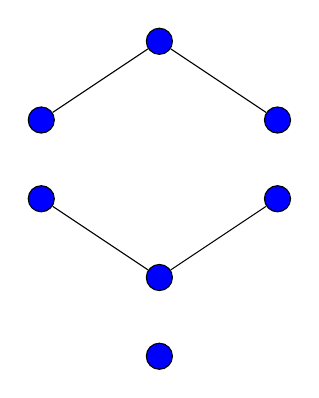
\begin{tikzpicture}[x=1.5cm,y=1cm,every node/.style={draw,solid,shape=circle,fill=blue}]

  % Specification of nodes (position, etc.)
  \node (a0) at (0,0) {};
  \node (b0) at (-1,-1) {};
  \node (b1) at (1,-1) {};
  \node (g0) at (-1,-2) {};
  \node (g1) at (1,-2) {};
  \node (j) at (0,-3) {};
  \node (c) at (0,-4) {};

  \begin{scope}[-]
    \tikzstyle{every node}=[draw,below]
    \draw[solid] (a0) to (b0);
    \draw[solid] (a0) to (b1);
    \draw[solid] (g0) to (j);
    \draw[solid] (g1) to (j);
  \end{scope}

\end{tikzpicture}
 };
    \node[scale=0.4] (state1a) at (4, 1.5) { 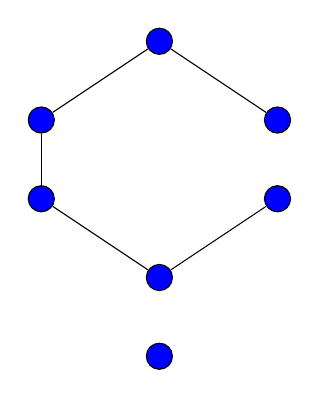
\begin{tikzpicture}[x=1.5cm,y=1cm,every node/.style={draw,shape=circle,fill=blue}]

  % Specification of nodes (position, etc.)
  \node (a0) at (0,0) {};
  \node (b0) at (-1,-1) {};
  \node (b1) at (1,-1) {};
  \node (g0) at (-1,-2) {};
  \node (g1) at (1,-2) {};
  \node (j) at (0,-3) {};
  \node (c) at (0,-4) {};

  \begin{scope}[-]
    \tikzstyle{every node}=[draw=none,below]
    \draw (a0) to (b0);
    \draw (a0) to (b1);
    \draw (b0) to (g0);
    \draw (g0) to (j);
    \draw (g1) to (j);
  \end{scope}

\end{tikzpicture}
 };
    \node[scale=0.4] (state1b) at (3, -1) { 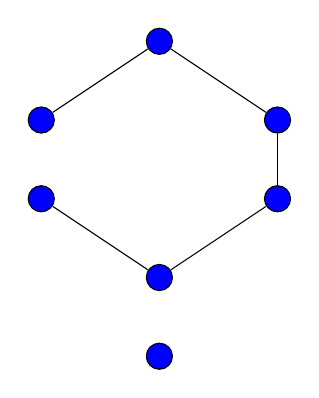
\begin{tikzpicture}[x=1.5cm,y=1cm,every node/.style={draw,shape=circle,fill=blue}]

  % Specification of nodes (position, etc.)
  \node (a0) at (0,0) {};
  \node (b0) at (-1,-1) {};
  \node (b1) at (1,-1) {};
  \node (g0) at (-1,-2) {};
  \node (g1) at (1,-2) {};
  \node (j) at (0,-3) {};
  \node (c) at (0,-4) {};

  \begin{scope}[-]
    \tikzstyle{every node}=[draw=none,below]
    \draw (a0) to (b0);
    \draw (a0) to (b1);
    \draw (b1) to (g1);
    \draw (g0) to (j);
    \draw (g1) to (j);
  \end{scope}

\end{tikzpicture}
 };
    \node[scale=0.4] (state2) at (4, -1) { 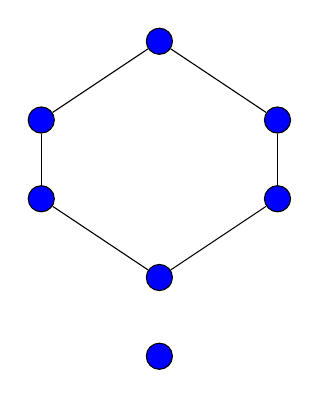
\begin{tikzpicture}[x=1.5cm,y=1cm,every node/.style={draw,shape=circle,fill=blue}]

  % Specification of nodes (position, etc.)
  \node (a0) at (0,0) {};
  \node (b0) at (-1,-1) {};
  \node (b1) at (1,-1) {};
  \node (g0) at (-1,-2) {};
  \node (g1) at (1,-2) {};
  \node (j) at (0,-3) {};
  \node (c) at (0,-4) {};

  \begin{scope}[-]
    \tikzstyle{every node}=[draw=none,below]
    \draw (a0) to (b0);
    \draw (a0) to (b1);
    \draw (b0) to (g0);
    \draw (b1) to (g1);
    \draw (g0) to (j);
    \draw (g1) to (j);
  \end{scope}

\end{tikzpicture}
 };
    \node[scale=0.4, rectangle, draw, dashed, rounded corners] (state3) at (4, -3.5) { 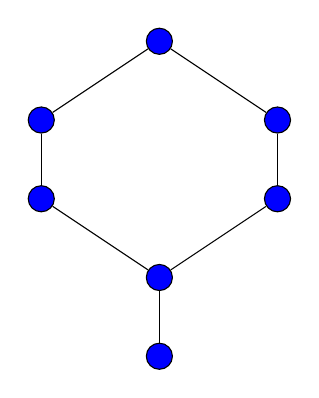
\begin{tikzpicture}[x=1.5cm,y=1cm,every node/.style={draw,solid,shape=circle,fill=blue}]

  % Specification of nodes (position, etc.)
  \node (a0) at (0,0) {};
  \node (b0) at (-1,-1) {};
  \node (b1) at (1,-1) {};
  \node (g0) at (-1,-2) {};
  \node (g1) at (1,-2) {};
  \node (j) at (0,-3) {};
  \node (c) at (0,-4) {};

  \begin{scope}[-]
    \tikzstyle{every node}=[draw=none,below]
    \draw[solid] (a0) to (b0);
    \draw[solid] (a0) to (b1);
    \draw[solid] (b0) to (g0);
    \draw[solid] (b1) to (g1);
    \draw[solid] (g0) to (j);
    \draw[solid] (g1) to (j);
    \draw[solid] (j) to (c);
  \end{scope}

\end{tikzpicture}
 };
    \node (expanded3) at (1, -6) { \begin{tikzpicture}[x=2.4cm, y=1cm, framed, background rectangle/.style={draw=black,dashed, rounded corners}] 

  % Specification of nodes (position, etc.)
  \node (a0) at (0,0) { $\adj{\alpha_L(x)\alpha_{L'}(x)}$ };
  \node (b0) at (-1,-1) { $\enf{\beta_L(G: x)}_{A, C}$ };
  \node (b1) at (1,-1) { $\enf{\beta_{L'}(G': x)}_{B, C}$ };
  \node (g0) at (-1,-2) { $\enf{\gamma_{G, J}(\rchi, A, C)}_{A, C}$ };
  \node (g1) at (1,-2) { $\enf{\gamma_{G', J}(\rchi, B, C)}_{B, C}$ };
  \node (j) at (0,-3) { $\enf{\beta_J(\rchi: x, C: x)}_{A,B,C}$ };
  \node (c) at (0,-4) { $\enf{\beta_\rchi(A: a, B: b)}_{A,B}$ };

  \begin{scope}[-]
    \tikzstyle{every node}=[draw=none,below]
    \draw (a0) to (b0);
    \draw (a0) to (b1);
    \draw (b0) to (g0);
    \draw (b1) to (g1);
    \draw (g0) to (j);
    \draw (g1) to (j);
    \draw (j) to (c);
  \end{scope}

\end{tikzpicture}
 };

    \begin{scope}[ultra thick]
      \tikzstyle{every node}=[below]
      \draw[-{Latex[length=3mm,width=4mm]}] (state0) edge (state1a)
                (state0) edge (state1b)
                (state1a) edge (state2)
                (state1b) edge (state2)
                (state2) edge (state3);
    \end{scope}
  \end{tikzpicture}
  \caption{Ledger channels, $x = a + b$}
  \label{fig:modes}
\end{figure} 
